\ifx\isEmbedded\undefined

\documentclass[12pt]{report}
\usepackage{tikz}
% FONT RELATED
%\usepackage{times} %Move to times font
\usepackage[labelfont=bf,textfont=it]{caption}

% LINKS, PAGE OF CONTENT, REF AND CROSS-REF, HEADERS/FOOTERS
\usepackage{hyperref}
\usepackage{fancyhdr}



% FIGURES, GRAPHICS, TABLES
%\usepackage{subfig}

%\usepackage{graphicx}
\usepackage{parskip}
%\usepackage{subfigure}
%\usepackage[dvips]{graphicx}
%\usepackage{pgfkeys}% gantt chart
\usepackage{lscape}
\usepackage{rotating}

% Algorithms
%\usepackage[ruled]{algorithm2e}

% COLOURS, TEXT AND FORMATTING
\usepackage{array}
\usepackage{color}
\usepackage{setspace}
\usepackage{longtable}
\usepackage{multirow}

% ADVANCED MATHS, PSEUDO-CODE
\usepackage{amsmath}
\usepackage{amssymb}
\usepackage{alltt}
\usepackage{gensymb}

% GANTT

\usepackage{pgfgantt}

% algorithm
\usepackage{algorithm,algpseudocode}
\usepackage{algorithmicx}

\usepackage{subfig}


\usepackage{adjustbox}

% BIBLIOGRAPHY
\usepackage[authoryear]{natbib}
\bibpunct{[}{]}{;}{a}{}{,}

% USE IN DISSER:

\setlength\oddsidemargin{1.5cm}
\setlength\evensidemargin{5cm}

\setlength\textheight{9.0in}
\setlength\textwidth{5.1in}

% indent at each new paragrapg
\setlength\parindent{0.5cm}

\setlength\topmargin{-0.2in}
\renewcommand{\baselinestretch}{1.3}



%REPORT
\algdef{SE}[DOWHILE]{Do}{doWhile}{\algorithmicdo}[1]{\algorithmicwhile\ #1}%
\newcommand{\HRule}{\rule{\linewidth}{0.0mm}}
\newcommand{\argmin}{\operatornamewithlimits{argmin}}
\newcommand{\argmax}{\operatornamewithlimits{argmax}}
% Color definitions (RGB model)
\definecolor{ms-comment}{rgb}{0.1, 0.4, 0.1}
\definecolor{ms-question}{rgb}{0.4, 0.0, 0.0}
\definecolor{ms-new}{rgb}{0.2, 0.4, 0.8}


\begin{document}
\fi
\chapter{3D Geometric Deformation}
\label{chap:landmark}
3D geometric deformation plays a key role in computer graphics and computer vision, and is the cornerstone of computer animation used in computer games and films. Large deformation is a challenging problem as it tend to produce stretch and shear on the shape, meanwhile, appropriate adjustment on local scale is required to adapt to the size difference. The mesh-connectivity on the deformable shape is supposed to be maintained as the users interactively editing the shape, but in the context of large deformation, they are susceptive to change as the distortion and scale may be easily brought into.

In the last two decades, there have been plenty of methods proposed on surface editing research aiming to solve these problem. However, these approaches either is unable to handle large deformation or suffer from fold-over due to their inconsitent energy. In this chapter, we will propose a novel deformation algorithm which not only is capable of addressing shapes with large difference in size but also ascertain a consistent energy to reduce the chance of fold-over and self-intersection. In this chapter we will introduce our consistent as-similar-as-possible (CASAP) deformation technique that not only is able to handle large deformation but also well preserve the mesh-connectivity.


%In the last two decades, there have been plenty of methods proposed on surface editing research aiming at preserve the mesh-connectivity and minimize the distortion. \cite{sorkine2007rigid} propose an as-rigid-as-possible (ARAP) surface modeling technique whose purpose is to maintain the local rigidity of the surface during deformation. The discrete cell adopt in as-rigid-as-possible deformation technique is a spokes, however, this method requires the use of a positive weighting scheme to guarantee the correct minimization of the energy. Chao et al.~\cite{chao2010simple} take into account all the opposite edges in the triangles incident to a vertex, the discrete cell in their work is a spokes and rims. Compared with ARAP deformation, this technique is guaranteed to always correctly minimize the energy even if the the weights are negative. However, the discretization of~\cite{chao2010simple} is only \emph{consistent} for volumetric case with tetrahedron cells in 3D or parameterization with triangle cells in 2D, it is not \emph{consistent} for the surface case with spokes and rims cells in 3D. In order to come up with a \emph{consistent} discretization for surface in 3D, \cite{levi2015smooth} introduce a new ARAP-type energy, named SR-ARAP (ARAP with smooth rotations), they add a bending term onto the ARAP energy to enable the discretization \emph{consistent}. \cite{yamazaki2013non} propose as-similar-as-possible (ASAP) energy in their work, which is able to deal with large difference in size and pose but the energy itself is not consistent leading to susceptive to fold-over and self-intersection. Therefore, designing an as-similar-as-possible and consistent energy is desirable.

\section{Notation and related methods}
Before stepping into the problem, we first introduce some basic concepts and notations of deformation which will be used in this research. We denote by $\mathcal S$ a triangle mesh. The piecewise linear geometric embedding of $\mathcal S$ is defined by the vertex positions $ \mathbf{p} \in \mathbf R^3$. Assume $\mathcal S$ is being deformed into $\mathcal S'$ that has the same connectivity and a different geometric embedding $\mathbf{p'}$. The discrete cell corresponding to vertex $i$ is denoted by $\mathcal  C_i$ and its deformed version $\mathcal  C'_i$. $\mathcal{E}_i$ is the corresponding edge sets in the cell $\mathcal  C_i$.

\cite{sorkine2007rigid} propose an as-rigid-as-possible energy to measure the local rigidity variation, in which the neighboring edge sets adopted are spokes. Given two meshes $\mathcal S$ and $\mathcal S'$ consisting of vertices $\mathbf{p}$ and $\mathbf{p'}$ respectively, the discrete ARAP energy between these two meshes is defined as:
\begin{equation}\label{earap}
E_{ARAP}(\mathcal S, \mathcal S')=\displaystyle \sum_i\!\!\sum_{(j,k)\in\mathcal{E}_i}\!\!\!w_{jk}\|(\mathbf p'_j - \mathbf p'_k)\!-\!\mathbf R_i(\mathbf p_j - \mathbf p_k)\|^2,
\end{equation}
where $w_{jk}$ are weighting coefficients, $\mathbf R_i \in RO(3)$ are optimal local rotation matrices. In the shape deformation setup, deforming a mesh $\mathcal S$ involves fixing handle points and solving for the rest of the $\mathbf{p'}$ by minimizing \eqref{earap}. The intuition for minimizing the ARAP energy is to find a mesh $\mathcal S'$ that is locally a rigid transformation of the source mesh $\mathcal S$. More specifically, the differential of a mapping from an edge set in $\mathcal S$ to a corresponding edge set in $\mathcal S'$ should be optimally a rotation, thus synchronizing corresponding edge vectors of the two edge sets.

Although ARAP shape deformation gained popularity, the energy is not consistent as it lacks a term measuring bending energy. \cite{levi2015smooth} introduce a new ARAP-type enery, named SR-ARAP (ARAP with smooth rotaions). The new energy used for surface deformation is consistent and can produce results with quality that competes with the volume deformation. They add a smoothing term to the ARAP surface energy to penalize the difference between the map differential of an edge set and the map differential of its neighboring edge sets. The SR-ARAP energy is defined as:
\begin{equation}\label{esrarap}
E_{\!S\!R\!-\!A\!R\!A\!P\!}(\mathcal S, \mathcal S')=\displaystyle \sum_i\!\!\sum_{(j,k)\in\mathcal{E}_i}\!\!\!w_{jk}\|(\mathbf p'_j - \mathbf p'_k)\!-\!\mathbf R_i(\mathbf p_j - \mathbf p_k)\|^2 + \alpha A\!\!\!\!\sum_{\mathcal{E}_l \in \mathcal{N}(\mathcal{E}_i)}\!\!\!\!\!\!w_{il}\|\mathbf R_i-\mathbf R_l\|_F^2 ,
\end{equation}
where $\mathcal{N}(\mathcal{E}_i)$ are the neighboring edge sets of $\mathcal{E}_i$;  $\alpha$ is a weighting coefficient; $A$ is the area of the whole mesh surface, which is used to make the energy scale invariant (scaling the edges by $s$, would scale the first term by $s^2$, which is the scale of $A$ in the second term); $w_{il}$ is scalar weight; $\|\cdot\|_F$ denotes the Frobenius norm. The second term is the bending energy, which penalizes the rigidity difference between a cell and its neighboring cells. In this way, they have made up the missing bending energy in ARAP to form a \emph{consistent} one.

Although SR-ARAP energy overcomes weaknesses in the ARAP surface deformation, which achieves the consistent discretization for the surfaces, it is still not capable of handling surfaces with different sizes since it aims at preserving the local rigidity of each cell. \cite{yamazaki2013non} propose an as-similar-as-possible energy to measure the local similarity variation, they add a freedom to the differential of a mapping with an isotropic scale $s_i$, which enables the energy to allow local scale to each discrete cell leading to capable to handling large size difference. The ASAP energy is defined as:
\begin{equation}\label{easap}
E_{ARAP}(\mathcal S, \mathcal S')=\displaystyle \sum_i\!\!\sum_{(j,k)\in\mathcal{E}_i}\!\!\!w_{jk}\|(\mathbf p'_j - \mathbf p'_k)\!-\!s_i\mathbf R_i(\mathbf p_j - \mathbf p_k)\|^2,
\end{equation}
 However, similar to ARAP energy, ASAP energy is also not consistent, which results in susceptive to fold-over and self-intersection.

In order to tackle the problems mentioned above, we propose a novel consistent energy called consistent as-similar-as-possible (CASAP) energy by introducing local scaling to the rotation in the prior SR-ARAP energy. It deforms surface meshes in an as-similar-as-possible manner, which is not only able to handle shapes with different size, but also reduce the occurrence of fold-over and self-intersection.

%===========================================================
\section{Consistent ASAP energy}
Assuming we are deforming a mesh $\mathcal S$ into $\mathcal S'$ in an as similar as possible way, unlike~\citep{sorkine2007rigid,yamazaki2013non,yoshiyasu2014conformal} regarding spokes as the edge sets, the edge sets chosen in this research is spokes and rims (denoted as $\mathcal{E}_i$) in order to arrive at an analyzable energy~\cite{chao2010simple}. If the deformation $\mathcal C_i \rightarrow \mathcal  C'_i$ is similar, then there exists a scale factor $s_i > 0$ and a rotation matrix $\mathbf R_i$ such that
\begin{equation}
\mathbf p'_j - \mathbf p'_k = s_i\mathbf R_i(\mathbf p_j - \mathbf p_k), \forall (j,k) \in \mathcal{E}_i,
\end{equation}
where $\mathcal{E}_i$ consists of the set of edges incident to vertex $i$ (the spokes) and the set of edges in the loop (the rims) of vertex $i$ in the surface mesh $\mathcal S$. When the deformation is not similar, we can still find the best approximating scale factor $s_i$ and rotation $\mathbf R_i$ by minimizing a weighted cost function
\begin{equation}
E(C_i,C'_i)=\sum_{(j,k)\in\mathcal{E}_i}w_{jk}\|(\mathbf  p'_j - \mathbf p'_k)-s_i\mathbf R_i(\mathbf  p_j - \mathbf p_k)\|^2,
\end{equation}
where $w_{jk}$ is thes edge weighting coefficient.

In order to measure the similarity of a deformation of the whole mesh, we sum up over the deviations from similarity per cell which yields us following ASAP energy functional:
\begin{align}
E_{ASAP}(\mathcal S, \mathcal S')&=\sum_i E(\mathcal  C_i, \mathcal C'_i)&=\displaystyle \sum_i\!\!\sum_{(j,k)\in\mathcal{E}_i}\!\!\!w_{jk}\|(\mathbf p'_j - \mathbf p'_k)\!-\!s_i\!\mathbf R_i(\mathbf p_j - \mathbf p_k)\|^2.\label{easap1}
\end{align}

However, according to~\cite{chao2010simple}, the ASAP energy we obtained so far is not \emph{consistent} yet. In fact, the resulting ASAP energy differs from the continuous one by a bending term. Inspired by~\cite{levi2015smooth} we incorporate the smooth regularization into \eqref{easap1} leading us to a \emph{consistent} ASAP energy:
\begin{align}
E_{\!C\!A\!S\!A\!P\!}(\mathcal S\!,\! \mathcal S'\!)\!\!=\!\!\displaystyle \sum_i\!(\!\!\!\sum_{(j,k)\in\mathcal{E}_i}\!\!\!\!w_{jk}\|(\mathbf p'_j\!\! -\!\! \mathbf p'_k)\!\!-\!\!s_i\!\mathbf R_i(\mathbf p_j - \mathbf p_k)\|^2\!\! +\!\!\alpha A\!\!\!\!\sum_{\mathcal{E}_l \in \mathcal{N}(\mathcal{E}_i)}\!\!\!\!\!\!w_{il}\|\mathbf R_i\!\!-\!\!\mathbf R_l\|_F^2 ),\label{ecasap}
\end{align}
where $\mathcal{N}(\mathcal{E}_i)$ are the neighboring edge sets of $\mathcal{E}_i$. The second term we add is the bending energy~\cite{levi2015smooth}, which penalizes the similarity difference between a vertex and its neighboring vertex. In this way, we have made up the missing bending energy in ASAP energy to form a \emph{consistent} one (Figure \ref{fig:consistent}).
\begin{figure}[h!tb]
	\begin{center}
			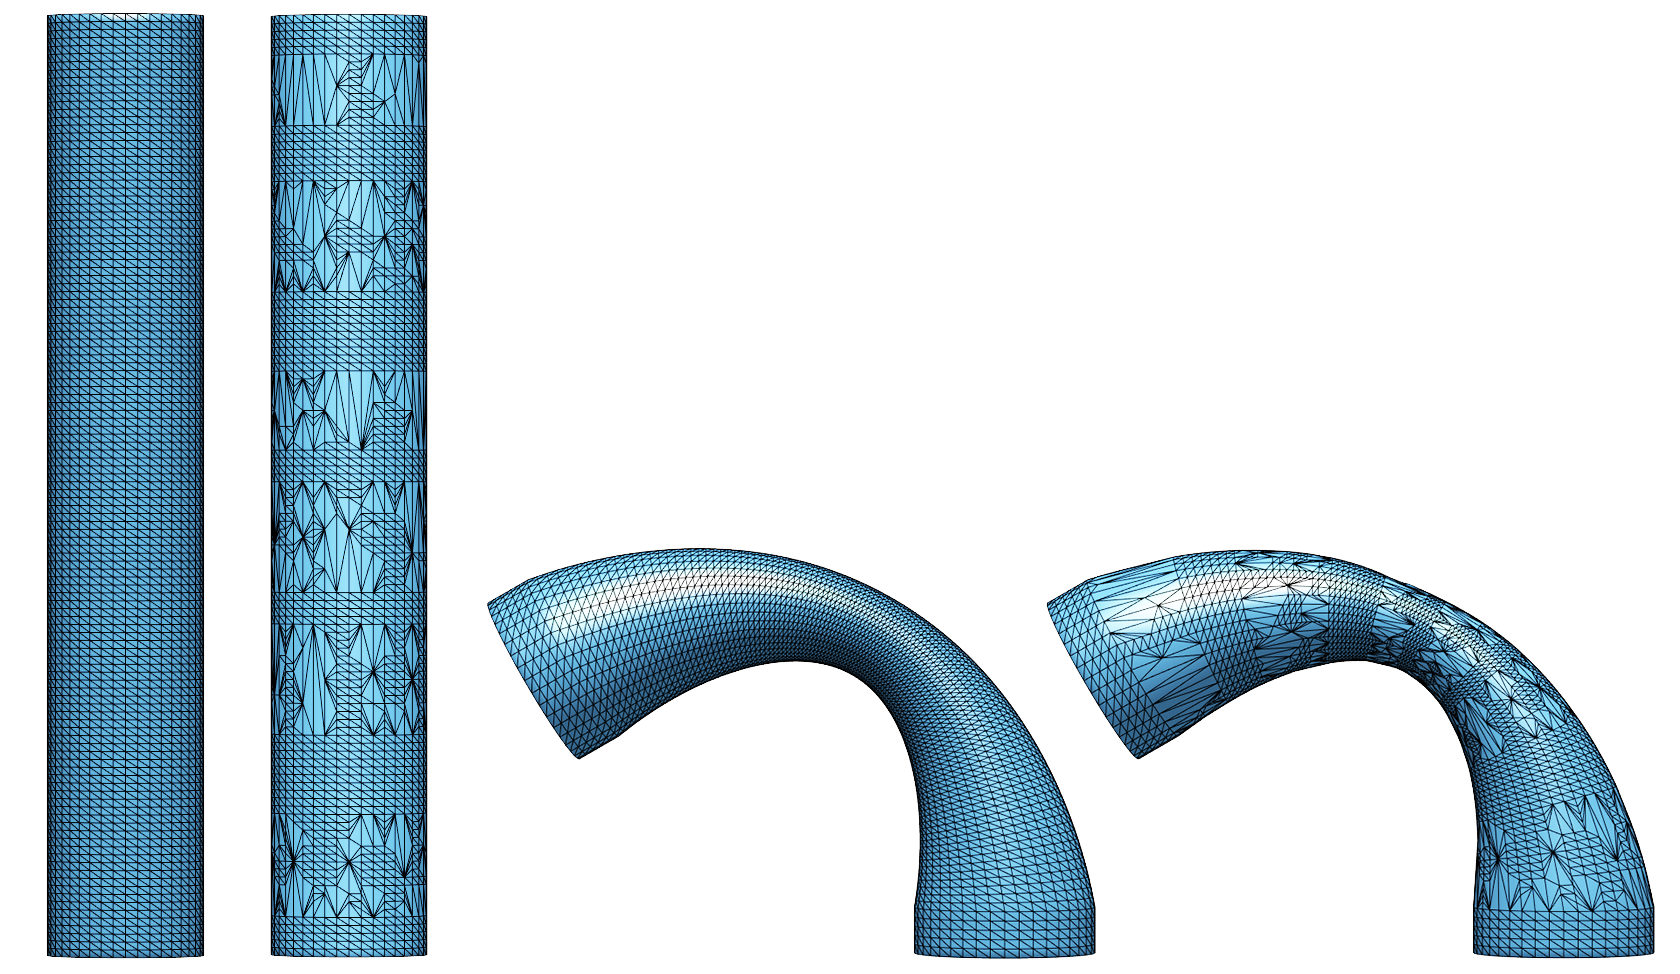
\includegraphics[width=0.9\columnwidth]{./figure/consistent_display.png}
	\end{center}
	\caption{CASAP deformation on the same object with different resolutions results in very similar qualitative behaviors.}
	\label{fig:consistent}
\end{figure}

%===========================================================

\section{Optimization}
In this subsection, we introduce the optimization algorithm to minimize the CASAP energy in \eqref{ecasap}. Note that except the vertex positions $\mathbf p_i$ are unknown, $s_i$ and $\mathbf R_i$ in \eqref{ecasap} are also unknown for each vertex. We employ the alternating optimization scheme following~\citep{sorkine2007rigid,yamazaki2013non,levi2015smooth} to solve them respectively. Each iteration consists of a local step followed by a global step. In local step, we optimize $s_i$ and $\mathbf R_i$ with $\mathbf p'_i$ fixed. By contrast, $\mathbf p'_i$ are optimized with $s_i$ and $\mathbf R_i$ fixed in global step.\\

$\textbf{Local}$ $\textbf{ step}$ ~~In this step, $\mathbf p'_i$ are fixed, and then we solve $\mathbf R_i$, $s_i$ in sequence to construct \emph{consistent} ASAP energy \eqref{ecasap}. For convenience, let us denote the edge $\mathbf e_{jk}:=\mathbf p_j-\mathbf p_k$ and $\mathbf e'_{jk}:=\mathbf p'_j-\mathbf p'_k$. Then we can change the formula \eqref{ecasap} for cell $i$ as
\begin{align}
\displaystyle \!\!\!\!\sum_{(j,k)\in\mathcal{E}_i}\!\!\!\!w_{jk}\|\mathbf e'_{jk}\!-\!s_i\!\mathbf R_i\mathbf e_{jk}\|^2\!+\!\alpha A\!\!\!\!\!\!\!\sum_{\mathcal{E}_l \in \mathcal{N}(\mathcal{E}_i)}\!\!\!\!\!\!w_{il}\|\mathbf R_i\!-\!\mathbf R_l\|_F^2 .\label{ecasapre}
\end{align}

First we solve for optimal rotation $\mathbf R_i$. Extending the equation \eqref{ecasapre} and dropping the terms that do not contain $\mathbf R_i$, we are remained with
\begin{align}
 &\argmin_{\mathbf R_i}~Tr(-\mathbf R_i(2\!\!\!\!\sum_{(j,k)\in\mathcal{E}_i}\!\!\!\!s_i\mathbf e_{jk}{\mathbf e'_{jk}}\!\!^T\!\!+\!2\alpha A\!\!\!\!\!\sum_{\mathcal{E}_l \in \mathcal{N}(\mathcal{E}_i)}\!\!\!\!\!\!w_{il}\mathbf R_l^T)) \nonumber\\
  &=\argmax_{\mathbf R_i}~Tr(\mathbf R_i\mathbf S_i),
\end{align}
where $Tr$ is the trace of a matrix, $\mathbf S_i$ is defined as
\begin{align*}
\mathbf S_i = 2\!\!\!\sum_{(j,k)\in\mathcal{E}_i}\!\!s_i\mathbf e_{jk}{\mathbf e'_{jk}}\!\!^T+2\alpha A\!\!\!\sum_{\mathcal{E}_l \in \mathcal{N}(\mathcal{E}_i)}\!\!\!\!\!\!w_{il}\mathbf R_l^T.
\end{align*}
Following~\cite{sorkine2007rigid} we derive the optimal rotation $\mathbf R_i$ from the singular value decomposition of $\mathbf S_i = \mathbf U_i\mathbf \Sigma_i\mathbf V_i^T$:
\begin{equation}\label{R}
\mathbf R_i = \mathbf V_i\mathbf U_i^T.
\end{equation}
The determinate of a rotation matrix should be one, if $\det(\mathbf R_i)<0$ then we change the sign of the column of $\mathbf U_i$ corresponding to the smallest singular.\\

Then we compute scale factor $s_i$. Since the second term in \eqref{ecasapre} is independent with $s_i$, we only extend the first term and divide extended terms by $s_i$
\begin{align}
 \argmin_{s_i,\mathbf R_i} Tr(\!\!\!\!\sum_{(j,k)\in\mathcal{E}_i}\!\!\!w_{jk}(\frac{1}{s_i}\|\mathbf {e'}_{jk}\|^2\!-\!2\mathbf R_i\mathbf e_{jk}{\mathbf {e'}_{jk}}^T + \!s_i\|\mathbf e_{jk}\|^2)). \label{sR}
\end{align}
Taking derivative \eqref{sR} w.r.t. $s_i$ and letting the derivative to be zero yields
\begin{align}\label{s}
s_i = {\left(\frac{\displaystyle \sum_{(j,k)\in\mathcal{E}_i}w_{jk}\|\mathbf e'_{jk}\|^2}{\displaystyle \sum_{(j,k)\in\mathcal{E}_i}w_{jk}\|\mathbf e_{jk}\|^2}\right)}^{\frac{1}{2}}
\end{align}\\

$\textbf{Global}$ $\textbf{ step}$ ~~In this step, vertex positions $\mathbf p'_i$ are optimized from $s_i, \mathbf R_i$ obtained by the local step.

Taking partial derivative of \eqref{ecasap} w.r.t. the position $\mathbf p'_i$ (note that the second term has nothing to do with $\mathbf p'_i$), we arrive at
\begin{align}\label{pd}
\frac{\partial E(\mathbf p')}{\partial \mathbf p'_i} =&2 \sum_{j \in \mathcal{N}(i)}\!(\!w_{ij}(3(\mathbf p'_i\!-\!\mathbf p'_j\!)\!-\!(\!s_i\mathbf R_i\!+\!s_j\mathbf R_j\!+\!s_m\mathbf R_m\!)(\mathbf p_i\!-\!\mathbf p_j\!))\nonumber\\
&+\!w_{ji}(3(\mathbf p'_i\!-\!\mathbf p'_j\!)\!-\!(s_i\mathbf R_i\!+\!s_j\mathbf R_j\!+\!s_n\mathbf R_n\!)(\mathbf p_i\!-\!\mathbf p_j\!))),
\end{align}
where $\mathcal{N}(i)$ is one-ring neighbors of vertex $\mathbf p'_i$; $s_m, s_n$ and $\mathbf R_m, \mathbf R_n$ are the scaler factors and rotation matrices of the vertices $\mathbf p_m, \mathbf p_n$ which are the opposite vertices of the edge $\mathbf e_{ij}$. Setting partial derivative $\eqref{pd}$ to zero gives the following sparse linear system of equations:

\begin{align}\label{sls}
\sum_{j \in \mathcal{N}(i)}(w_{ij}\!+\!w_{ji})(\mathbf p'_i-\mathbf p'_j)=&\frac{1}{3}\!\sum_{j \in \mathcal{N}(i)}\!(w_{ij}(s_i \mathbf R_i\!+\!s_j\mathbf R_j\!+\!s_m \mathbf R_m\!)\! \nonumber\\
&+\!w_{ji}(s_i \mathbf R_i\!+\!s_j \mathbf R_j\!+\!s_n \mathbf R_n))(\mathbf p_i\!-\!\mathbf p_j\!).
\end{align}
Notice that the linear combination on the left-hand side is the discrete Laplace-Beltrami operator applied to $\mathbf p'$. Now the system of equations can be reduced as \begin{equation}\label{DeformationLinearSystem}
\mathbf L\mathbf p' = \mathbf d,
\end{equation} where $\mathbf L$ represents the discrete Laplace-Beltrami operator, which only depends on the initial mesh, thus it can be pre-factored for efficiency; $\mathbf d$ is given by the right-hand side of $\eqref{sls}$.\\

Up to now, the optimization of \emph{consistent} ASAP energy can be summarised as Algorithm \eqref{casapdeformational}.
\begin{algorithm}[]
\caption{\emph{Consistent} ASAP Energy Optimization}
\label{casapdeformational}
\begin{algorithmic}[1]
    \While{not converged}
        \State Compute $\mathbf R_i$ by solving equations \eqref{R}.
        \State Compute $s_i$ by solving equations \eqref{s}.
        \State Compute $\mathbf p'$ and update surface $\mathcal S'$ by solving equation \eqref{DeformationLinearSystem}.
    \EndWhile
\end{algorithmic}
\end{algorithm}

%===========================================================
\section{Experiments}
We compare our \emph{consistent as-similar-as-possible} (CASAP) deformation approach with other three deformation methods: ARAP~\citep{sorkine2007rigid}, SR-ARAP~\citep{levi2015smooth} and ASAP~\citep{yamazaki2013non}) in Figure \ref{fig:deformation_comparison}. The result of ARAP is not satisfying because its energy is not \emph{consistent}. SR-ARAP overcomes the weakness of ARAP, offering a \emph{consistent} energy. However, it cannot handle local scalability. ASAP allows piecewise scale but its energy is not \emph{consistent}, which may lead to undesirable results such as fold-over and self-intersection. CASAP combines the benefits of ASAP with the advantages of the SR-ARAP approach such that it can not only handle local scale but also guarantee the deformation smoothness. Moreover, in terms of isometric deformation, it produce competitive results as good as SR-ARAP. Figure \ref{fig:consistent} shows the advantages of our \emph{consistent} energy.\\
 \begin{figure}[!hptb]
 \centering

 \captionsetup[subfigure]{labelformat=empty}
 \centering

			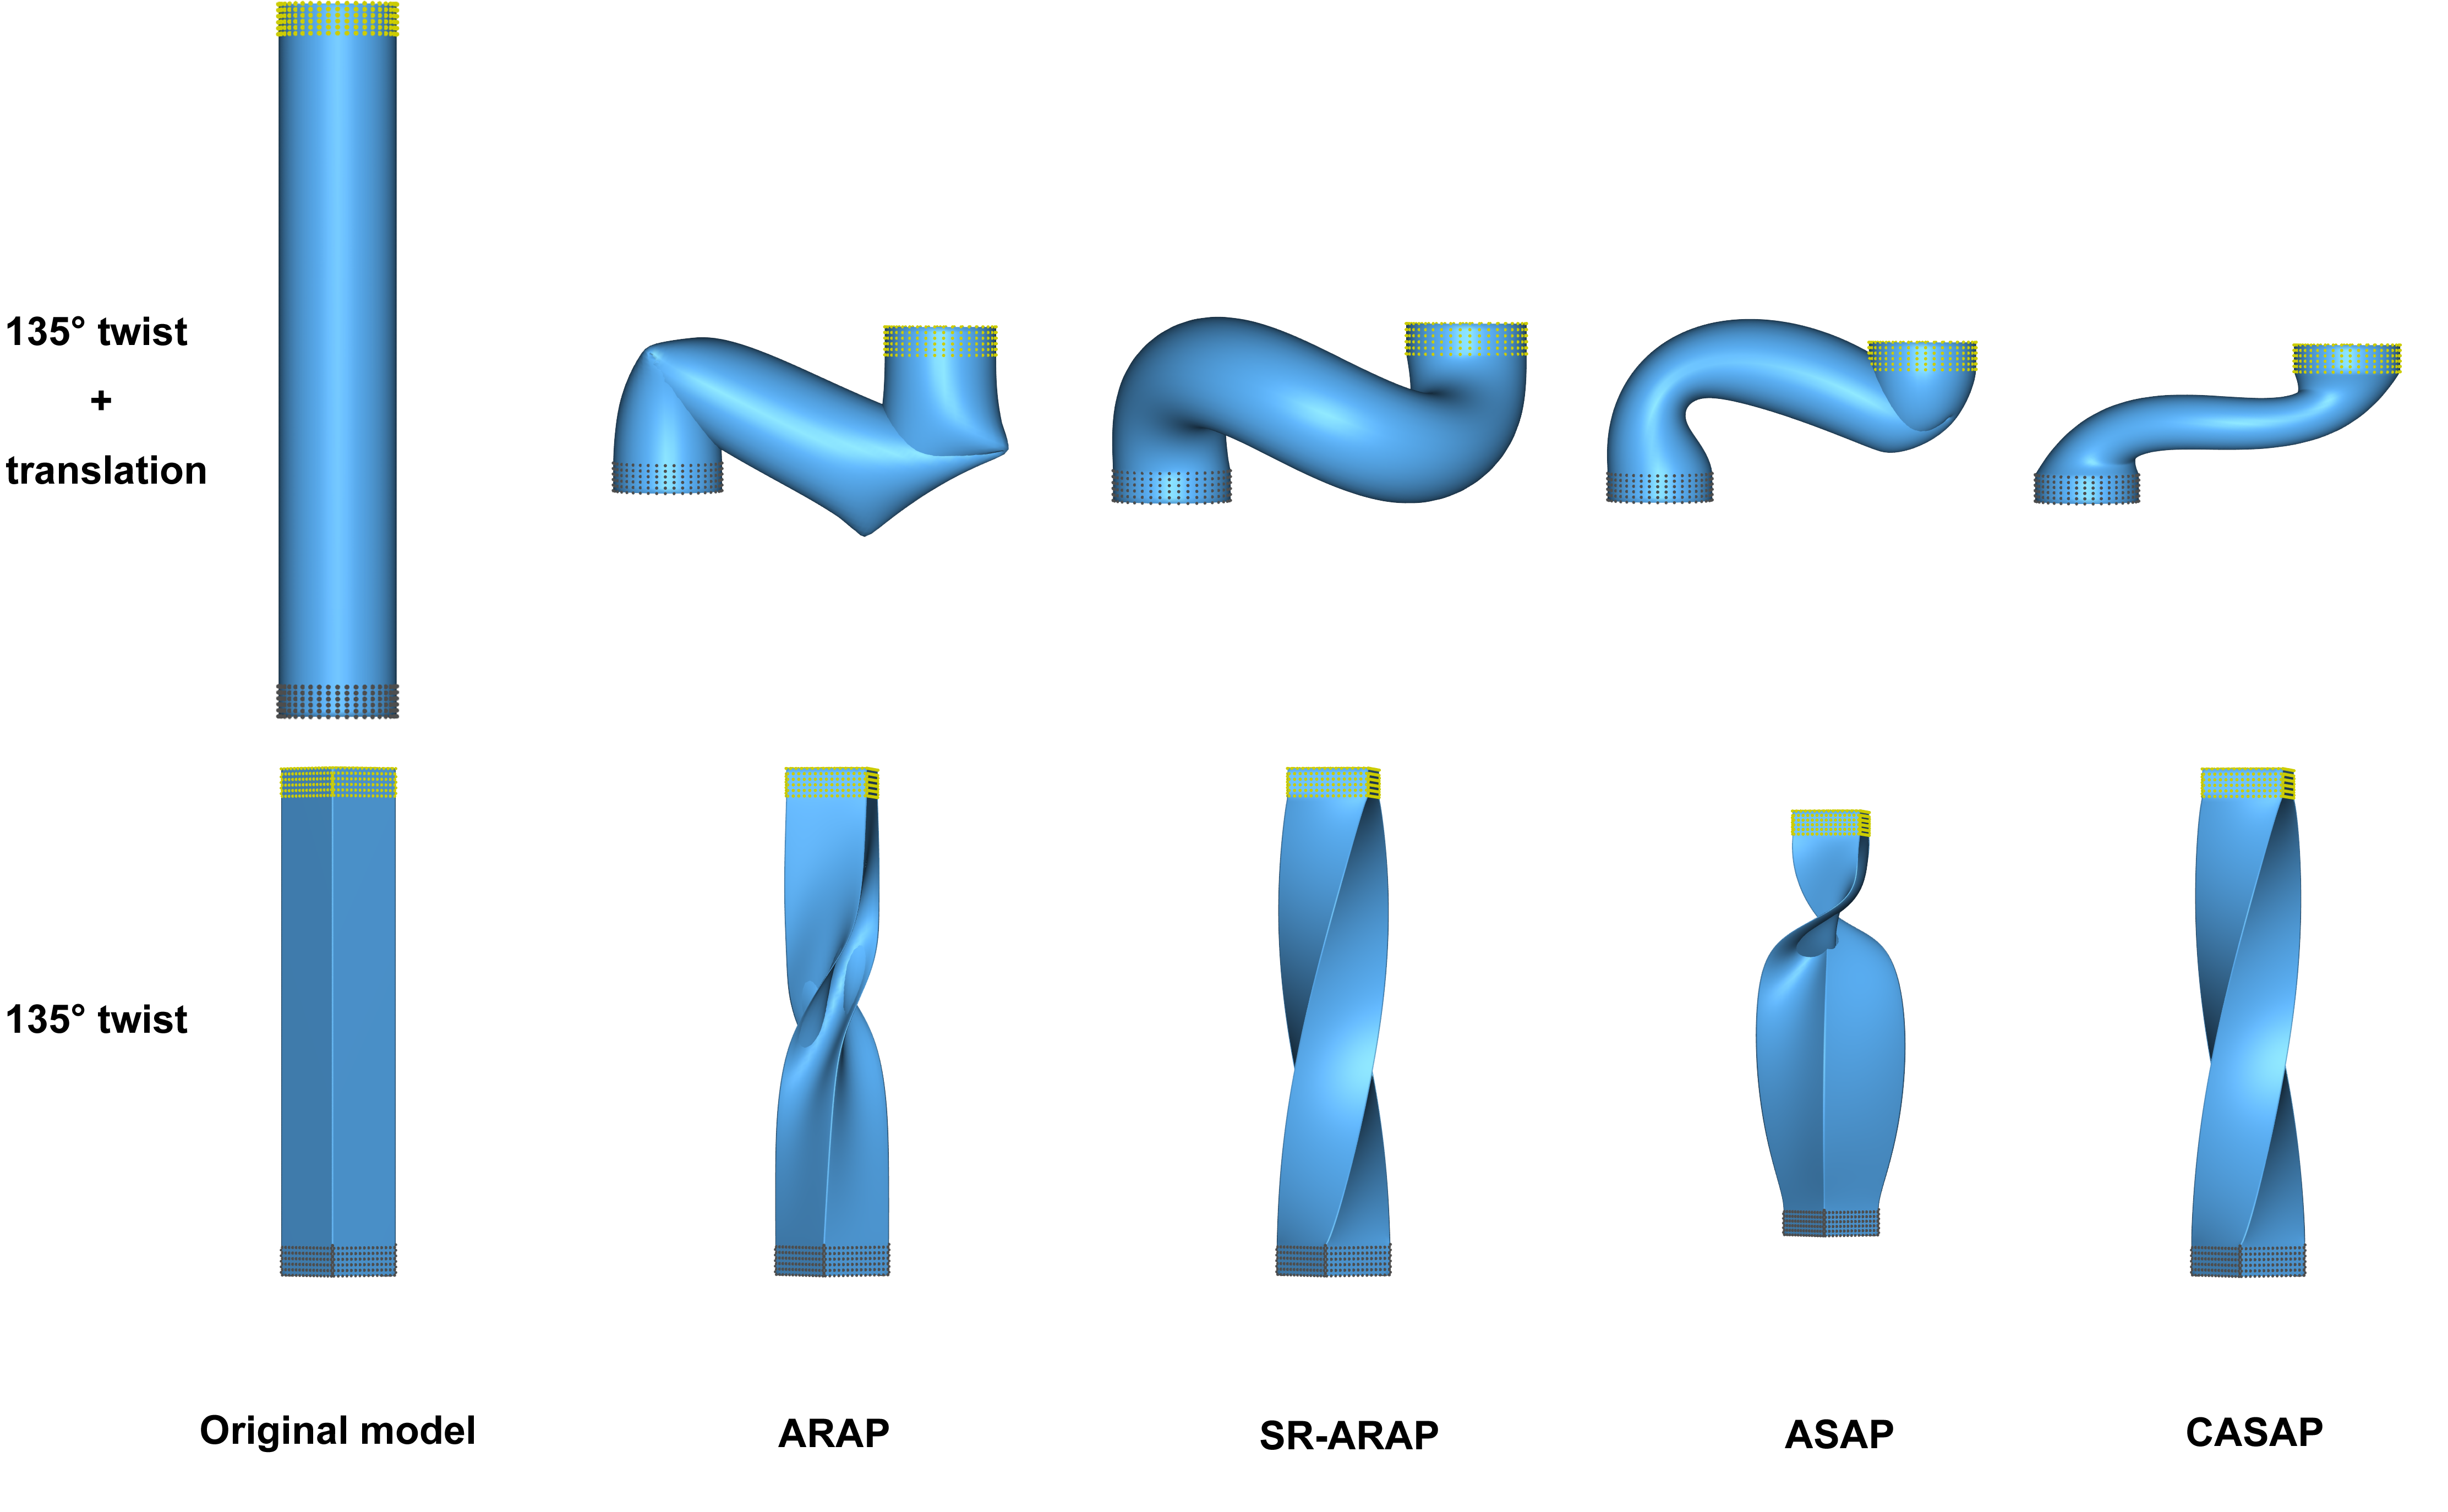
\includegraphics[width=\columnwidth]{./figure/deformation_comparison.png}


     \caption{Different deformation approaches comparison. Rows show different transformations, while columns represent different deformation methods. The grey points are fixed and the yellow ones indicate control points.  }
     \label{fig:deformation_comparison}
 \end{figure}
%===========================================================
\section{Conclusion}
We proposed a novel consistent as-similar-as-possible surface deformation method, which not only allows local scale to each discrete cell but also achieves the consistent discretization for surfaces. The important features of our approach are (1) robustness, resulting from the minimization procedure that is guaranteed to not increase energy in each step; (2) simplicity, as each iteration of the minimization solves a linear system; (3) efficiency, because the laplace system matrix is constant throughout the iterations and can be pre-factored just for once. We fitted the mapping differential into a similarity matrix, which is an isotropic scale factor times a rotation matrix. The scale factor is able to handle size difference while the rotation matrix part prevents local stretch and distortion. Meanwhile, the added rotation smoothing term compensates the bending energy which makes CASAP energy consistent, reducing the risk of fold-over and self-intersect occurrence. Our technique fills the missing gaps between SR-ARAP and ASAP. It combines the benefits of SR-ARAP and the advantage of ASAP, producing a consistent discretization and allowing local scalability to handle large deformation consistently without compromising the efficiency.




\ifx\isEmbedded\undefined
% References
\addcontentsline{toc}{chapter}{References}
\pagebreak
\end{document}
\fi
